\documentclass[tikz,border=10pt]{standalone}
\usepackage{tikz}
\usetikzlibrary{positioning}
\usetikzlibrary{shapes.geometric}% tikz node 形状的库
\usetikzlibrary{patterns}
\usepackage{tikz-feynman}
\begin{document}

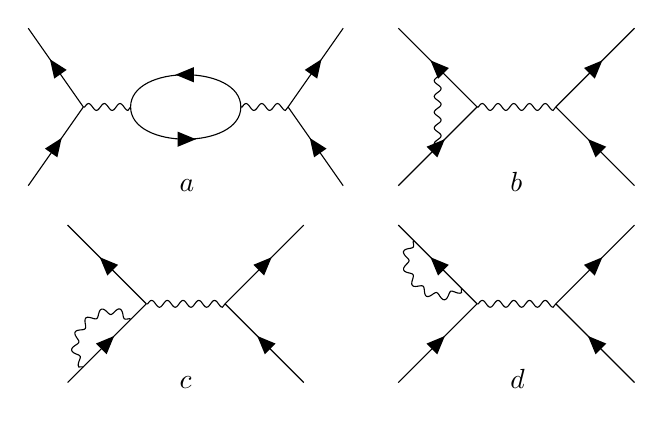
\begin{tikzpicture}
	\begin{feynman}
		%% fig a
		\vertex (a1) at (0,0);
		\vertex[above right = -2 and 0 of a1] (a2);
		\vertex[above right = 0 and 4 of a1] (a3);
		\vertex[above right = -2 and 4 of a1] (a4);
		\vertex[above right = -1 and .7 of a1] (a5);
		\vertex[above right = -1 and 3.3 of a1] (a6);
		\vertex[above right = -1 and 1.3 of a1] (a7);
		\vertex[above right = -1 and 2.7 of a1] (a8);
		\node[above right = -2.2 and 1.8 of a1] {\(a\)};
		% 对各个顶点连线
		\diagram*{
		(a2) --[fermion] (a5)--[fermion](a1);(a4) --[fermion] (a6)--[fermion](a3);
		(a5)--[photon](a7);(a8)--[photon](a6);
		(a7)--[half right,fermion,looseness=1](a8);(a8)--[half right,fermion,looseness=1](a7);
		};
	\end{feynman}
	\begin{feynman}[xshift=4.7cm]
		%% fig a
		\vertex (a1) at (0,0);
		\vertex[above right = -2 and 0 of a1] (a2);
		\vertex[above right = 0 and 3 of a1] (a3);
		\vertex[above right = -2 and 3 of a1] (a4);
		\vertex[above right = -1 and 1 of a1] (a5);
		\vertex[above right = -1 and 2 of a1] (a6);
		\vertex[above right = -0.5 and 0.5 of a1] (a7);
		\vertex[above right = -1.5 and 0.5 of a1] (a8);
		\node[above right = -2.2 and 1.3 of a1] {\(b\)};
		% 对各个顶点连线
		\diagram*{
		(a2) --[fermion] (a5)--[fermion](a1);(a4) --[fermion] (a6)--[fermion](a3);
		(a5)--[photon](a6);(a7)--[photon](a8);
		};
	\end{feynman}
	\begin{feynman}[xshift=.5cm,yshift=-2.5cm]
		%% fig a
		\vertex (a1) at (0,0);
		\vertex[above right = -2 and 0 of a1] (a2);
		\vertex[above right = 0 and 3 of a1] (a3);
		\vertex[above right = -2 and 3 of a1] (a4);
		\vertex[above right = -1 and 1 of a1] (a5);
		\vertex[above right = -1 and 2 of a1] (a6);
		\vertex[above right = -1.2 and 0.8 of a1] (a7);
		\vertex[above right = -1.8 and 0.2 of a1] (a8);
		\node[above right = -2.2 and 1.3 of a1] {\(c\)};
		% 对各个顶点连线
		\diagram*{
		(a2) --[fermion] (a5)--[fermion](a1);(a4) --[fermion] (a6)--[fermion](a3);
		(a5)--[photon](a6);
		(a7)--[half right,photon,looseness=1.5](a8);
		};
	\end{feynman}
	\begin{feynman}[xshift=4.7cm,yshift=-2.5cm]
		%% fig a
		\vertex (a1) at (0,0);
		\vertex[above right = -2 and 0 of a1] (a2);
		\vertex[above right = 0 and 3 of a1] (a3);
		\vertex[above right = -2 and 3 of a1] (a4);
		\vertex[above right = -1 and 1 of a1] (a5);
		\vertex[above right = -1 and 2 of a1] (a6);
		\vertex[above right = -.2 and 0.2 of a1] (a7);
		\vertex[above right = -.8 and 0.8 of a1] (a8);
		\node[above right = -2.2 and 1.3 of a1] {\(d\)};
		% 对各个顶点连线
		\diagram*{
		(a2) --[fermion] (a5)--[fermion](a1);(a4) --[fermion] (a6)--[fermion](a3);
		(a5)--[photon](a6);
		(a7)--[half right,photon,looseness=1.5](a8);
		};
	\end{feynman}
\end{tikzpicture}

\end{document}